\label{key}%\documentclass{template/openetcs_article}
% Use the option "nocc" if the document is not licensed under Creative Commons
%\documentclass[nocc]{template/openetcs_article} 
%\documentclass[nocc]{template/openetcs_article}
\documentclass{template/openetcs_report}
\usepackage{lipsum,url}
\usepackage{xspace}
\usepackage{graphicx}
\usepackage{fixme}
\usepackage{lscape} 
\usepackage{pgfgantt}
\usepackage{adjustbox}
\usepackage{datetime}
\usepackage{wrapfig}


%user specified macros
%\input{macros.tex}

\graphicspath{{./template/}{.}{./images/}{./bilder/}}
\begin{document}
\frontmatter
\project{openETCS}

%Please do not change anything above this line
%============================
% The document metadata is defined below

%assign a report number here
\reportnum{OETCS/WP3/Brussels/WS/Minutes}

%define your workpackage here
\wp{Work Package 3: ``Modelling and Code generation''}

%set a title here
\title{openETCS Modelling Work Package}

%set a subtitle here
\subtitle{Workshop in Brussels}

%set the date of the report here
\date{26 - 28 Mai 2014}

%define a list of authors and their affiliation here

\author{openETCS WP3 SRS task force}

%\affiliation{The Team}
 
\author{Jacques Por\'e}

%\affiliation{WP3 Safety and Requirements Traceability}

\author{Fausto Cochetti}

\affiliation{WP3}

% define the coverart
\coverart[width=350pt]{openETCS_EUPL}

%define the type of report
\reporttype{Minutes of meeting}



\begin{abstract}
%define an abstract here

  This document resumes the items presented during the WP3 meeting in Brussels 26 to 28 May 2014. Venue: ALSTOM Transport Brussels,
  Place Marcel Broodthaerts 8/b 3  -  1060 Brussels (phone: +32 (0)71 44 56 08)
  (close to Brussels Midi railway station)



\end{abstract}

%=============================
%Do not change the next three lines
\maketitle
\tableofcontents
\listoffiguresandtables
\newpage
%=============================

% The actual document starts below this line
%=============================


%Start here

\chapter*{Workshop {\bf ITEA OPEN ETCS WP3} on 26-28 May in Brussels, called up by Alstom}
%-----------------------------------------------------------------------
\section*{Attendees: }
%-----------------------------------------------------------------------
\begin{figure}[!ht]
%\boxed{
\centerline{
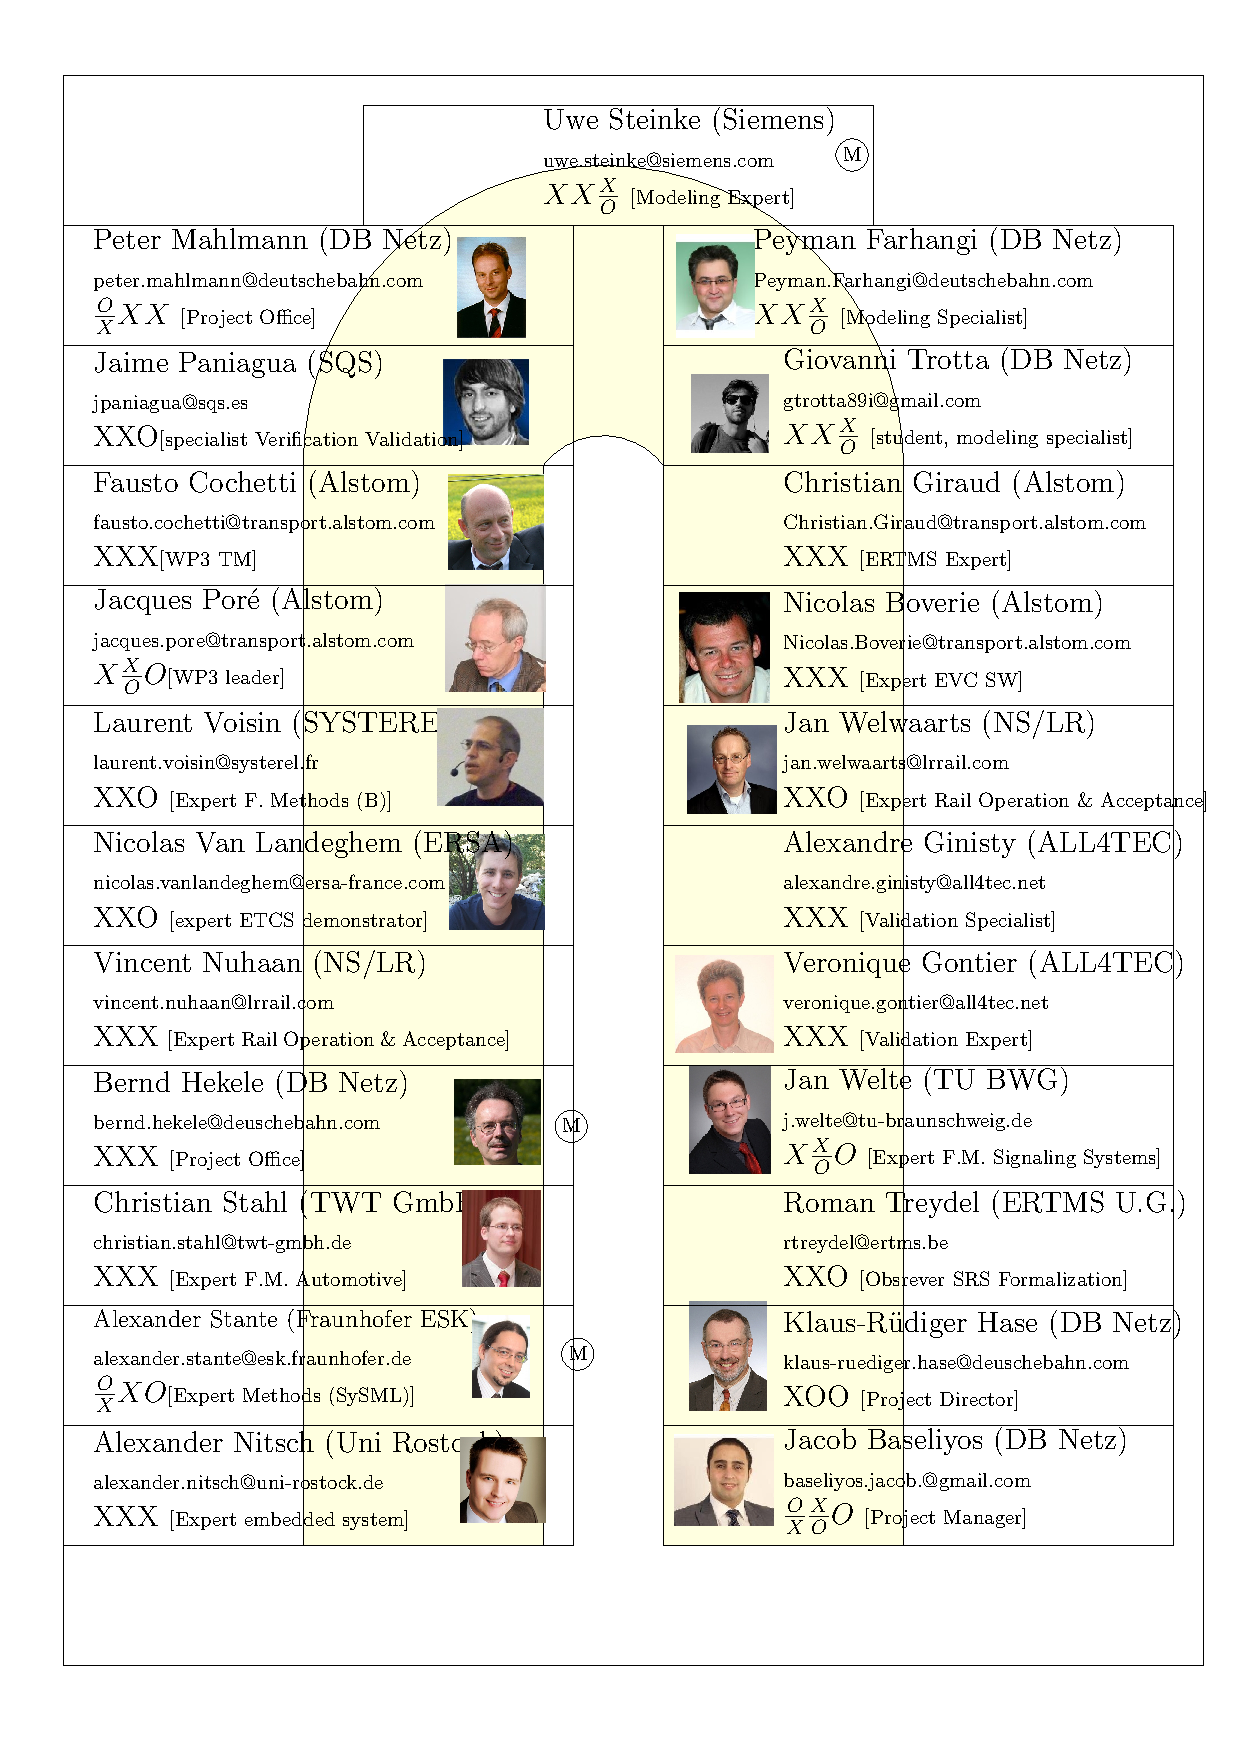
\includegraphics[angle=-0,width=.95\textwidth]{table2r.pdf}
}
%}
\caption{\emph{Participants around the table during the meeting}}
\label {fig:table}
\end{figure}

Companies and institutes represented have been:

\begin{itemize}
\item [-]ALL4TEC
\item [-]ALSTOM: Nicolas Boverie, API;
Fausto Cochetti, WP3 Deputy Leader and Alstom representative for the other WPs;
Christian Giraud, WP3 Technical Leader;
Jacques Por\'e, WP3 Leader.\footnote{
ALSTOM is an established railway supplier worldwide with experience in ERTMS/ETCS from the origins and experience in formal methods from the 1970s e.g. SACEM ATP for metros. Alstom is one of the contributing members of UNISIG and has actively contributed to the definition of the ERTMS standards and requirements.
ALSTOM has been involved in the Open ETCS from its start having agreed to become donor of the source code of the EVC according to the rules defined in the ICE contract with DB. Alstom is WP3 Leader in the Itea initiative related to the realization of an open proof platform and is active/present in all WPs. }
\item [-]DB: Klaus-R\"udiger Hase, OpenETCS Director; Bernd Hekele, OpenETCS project office;
Baseliyos Jacob, OpenETCS Project management.
Peyman Farhangi, OpenETCS modeling expert
Peter Mahlmann, OpenETCS modeling and wp management, Giovanni Trotta engineering student modeling specialist
\footnote{
DB, German Railways have been the promoter of OpenETCS and contributed to introduce new ways of working and tools, formal methods and the like in the development of ERTMS/ETCS with focus on on-board equipment.}
\item [-]ERSA
\item [-]ERTMS Users’ Group
\item [-]Fraunhofer
\item [-]NS/Lyods
\item [-]SIEMENS
\item [-]SQS
\item [-]SYSTEREL
\item [-]Technische Universit\"at Braunschweig
\item [-]TWT GmbH
\item [-] Universit\"at Rostock
\end{itemize}


\section{Reminder from the agenda}
\begin{itemize}
\item[-]Short presentation of each company/organization acting in WP3 and present at the workshop
\item[-]Reminder of the general context of the project and of the key role of activity within WP3. KRH
\item[-]presentation of general structure of repositories and procedures to access relevant information for the project BH.
\item[-]presentation of the technical document prepared by Alstom \emph{WG3\_OpenETCS\_Database\_V7.doc} CG.
\item[-]presentation of scope and architecture outlined for first iteration in Berlin during the previous Workshop in November 2013. US
\item[-]presentation of present status of the SW model implemented in the Scade-suite tool. Example of debugging session on Scade model. The Model (first iteration) will be completed by end of July. US
\item[-]outline of next steps to prepare for next iteration of SW model 
\item[-]installation of toolchain OpenETCS {\bf E}xtended {\bf T}ool {\bf C}onstruction {\bf S}et. The Scade tool beeing a non OSS requires a specific license to be operated and can therefore not be installed for now on new workstations.
\end{itemize}
\section{action plan and next steps}
\begin{itemize}
\item[+] Complete SCADE modeling according to scope defined in last Berlin Workshop (end of July)
\item[+]{Analyze new features introduced by Alstom Document \emph{OpenETCS\_Database}
In particular there is the need to analyze the variables and the data required and compare to the data-types already available in the modeling environment. Another important issue is related to the implementation in the modeling environment of the dynamic data structure essential for the processing and monitoring. }
\item[+] Define a basic scope to be viable for WP4
\item[+] Get a solution for making the API data available in the simulation environment
\item[+] Organize a technical Workshop End of June
\item[+] Prepare for an extended Workshop in September
\end{itemize}

\appendix
\chapter{Items of technical discussion}

\section{Reminder : modeling scope set up during last Berlin workshop}
\subsection{Essential Function to track train position}

The target “essential functionality to track a running train” in terms of on ETCS OBU : 
\begin{itemize}
	\item train moves on a track equipped with balises, OBU determines its position.
	\item train moves according to given predefined pattern or record. Movement is not influenced by OBU function.
	\item balise information are given as a predefined track tape e.g. as recorded by a real train.
\end{itemize}
OBU shall not supervise the maximum speed, shall not activate the brakes. The minimum function set shall be limited to (see \url{https://github.com/openETCS/SRS-Analysis/issues/9} ) 
\begin{itemize}
	\item Receive, filter and manage balise information, received from track (see \url{https://github.com/openETCS/SRS-Analysis/issues/12})
	\item Calculate the actual train position based on odometry + balise information (see \url{https://github.com/openETCS/SRS-Analysis/issues/8})
	\item Calculate the distances to relevant track elements of train according to required reference.
\end{itemize}

A more detailed architectural breakdown of these functions is available in the form of a SysML model at (see \url{https://github.com/openETCS/modeling/tree/master/model/sysml}). 

\section{Modeling evolution as exposed by Alstom}
\subsection{Data architecture and technical background for monitoring function}
Christian Giraud from Alstom introduced the technical document: \emph{WG3\_OpenETCS\_Database\_V7.doc}\footnote{Actually in the title page the WG3 should be replaced by WG2} with a dedicated presentation. Main content is around the choices for a SW modeling concept recapitulating main technical and physical aspects of the calculation and monitoring of a safe braking condition. In the document a specific data structure \emph{(database)} to store relevant data for a given train position sorted according to the train path coordinate is introduced. A draft architecture is also proposed. This SySML IBD preliminary diagram needs to be developed to the level of detail needed to be non ambiguous, integrating wherever possible all the steps already consolidated by the team during the preceding phase. Other relevant aspects which are covered by the document are the definition of the data (primary and optional) needed for implementing a safe movement elaboration, including the linking rules and the link matching truth table, which relates pending linking information (packet 5) with detected header link marker Q\_LINK and how to handle an process the data in chapter 4. In the final chapter 6 an exemplar calculations is performed in order to give an extensive overview of the complexity to be reached by the basic algorithms.

\begin{enumerate}
\item The State of the Art in terms of specification and applicable tools:
\begin{itemize}
\item[-] SCADE as part of a toolchain (SysML, Modeling, Formal Spec / runtime code generation)
\item[-] SysML  : Papyrus (visual modeling language)
\item[-] Algorithm Modeling : Excel (parametric modeling as used e.g. by the ERA braking curve tool)
\item[-] Formal Specifications : B 
\item[-] Runtime code : ADA / C++
\item[-] Other simulation tools for specific subtasks e.g. LabView, Simulink \ldots
\end{itemize}
\item Open design approach including reverse-engineering :
\begin{itemize}
\item[-] Word, Excel
\item[-] SysML method
\end{itemize}
\item Versus incremental approach step by step :
\begin{itemize}
\item[-]Balise reading
\item[-]Train position tracking
\item[-]Time stamp
\end{itemize}
\end{enumerate}

\subsection{Three step approach}
A gradual approach is suggested, divided in 3 main phases. In the first phase a formal breakdown of the application is performed, then in a second step this diagram is refined until a non ambiguous level is reached (library concept) and a selection of modules according to viable scope to perform a validation run is established. Finally the most complex functions are modeled in order to consolidate a retraceable specification.

\subsection{Discussion on a possible API strategy}
The API documented in the paper \emph{API requirements for OpenETCS - v1.2} is based on the HW and SW architecture of the Alstom EVC reflecting the Source code, that will be made available in Open ETCS contract with DB. Nevertheless in the frame of the Itea project it is desirable to refer to a vendor neutral API specification. It is foreseen to note the requirements for an API abstraction layer while the model will grow and corresponding adaptations will be needed. In the meantime it should be possible to maintain data-structures suitable or the running SW model within the cyclic scheduler of the Scade model. Main difference between the Scade SW model and the runtime API is related to the fact that the Scade model is operated in deterministic cycle while the runtime SW has to manage time sorting due to random time sliding effects.

\subsection{Application}
\begin{enumerate}
\item ThreePhases
\begin{itemize}
\item System Specification (Application software or Kernel)
\begin{itemize}
\item SysML
\begin{itemize}
\item[*]BDD (Block Definition Diagram)
\item[*]IBD (Internal Block Diagram)
\item[*]STM (State Machine)
\end{itemize}
\item Math and Boolean Equations
\begin{itemize}
\item[*] Model Simulation 
\end{itemize}
\item Deliver a Reference for V\&V phase
\item Programming language
\begin{itemize}
\item[*]ADA
\item[*]B
\item[*]C++
\end{itemize}
\end{itemize}
\end{itemize}

\item Architecture : reach a level of precision enabling to proceed to encoding,
\begin{itemize}
\item define a consistent perimeter for the iterative approach
\item 2-dimensional data structure for storing location based information
to store Singular points \footnote{Data sets associated to a specific position or track coordinate} :
\begin{itemize}
\item[-]BG
\item[-]MA  : section, EOA, DP, OL
\item[-]SSP (Static Speed Profile) change
\item[-]Grade change
\item[-]Optional track data (e.g. Level Transition, TSR, LX data)
\end{itemize}

\item To manage reordering (sorting) of  singular points according track position
\item To compute following values :
\begin{itemize}
\item[-]MRSP
\item[-]Target
\item[-]Energy per mass unit
\end{itemize}
\end{itemize}

\item  extended management of track data : 2-dimensional data structure (Virtual Machine)
\begin{itemize}
\item information sorted according to \emph{Track Layout}\footnote{measure along the rail constrained train path }
\item internal index that qualifies different parameters at a given location
\begin{itemize}
\item[1st column] : type
\item[2nd column] : position
\item[3rd column] : typical parameter
\item[4th column] : Asafe
\item[5th column] : Grade
\item[6th column] : SSP
\item[Next columns] computation of data :
\begin{itemize}
\item[-] MRSP
\item[-] Target
\item[-] residual energy per mass unit $\frac{m^2}{s^2}$
\end{itemize}
\end{itemize}
\end{itemize}
\end{enumerate}



\chapter{Items related to project infrastructure and organisation}
\section{Organisation of Repositories}

 Here is an overview on repositories containing content related to some of the arguments of the workshop.

\begin{itemize}
\item \url{https://github.com/openETCS/modeling}\\
The modeling repository is the place where modeling takes place. openETCS ToolChain is linked to this repository (folder "model". All code artefacts have to reside in this location. 


\item \url{https://github.com/openETCS/SRS-Analysis}\\
The SRS-Analysis Repository was introduced to support the task force dedicated to the analysis work.
 The repository is still in use.

\item \url{https://github.com/openETCS/dataDictionary}\\
The data-Dictionary repository is related to the definition of common data and functions. The dataDictionry implementation is based on SysML/Papyrus. No tools nor artefacts are stored here, only documentation. The repository is still in use.

\item \url{https://github.com/openETCS/SSRS}\\
The SSRS activities had been used before the modelling kick-off to prepare for the analysis work. There are stil some useful documents included. Especially the wiki is usefull.
The place is no longer used for active work. 

\item Requirements on Process and Methods, Guidelines\\
The following guidelines are the basis for modeling work:
The openETCS development process: \url{https://github.com/openETCS/requirements/blob/master/D2.3/D2_3.pdf}\\
The openETCS requirements on methods: \url{https://github.com/openETCS/requirements/blob/master/D2.4/D2_4.pdf} 
This document also describes naming conventions which you need to respect for working in this task.

\end{itemize}


%\input{sections/methodology.tex}

\section{Verification and Validation of Modeling artefacts}
The handling is based on the openETCS review process which is documented as an extension of the quality insurance plan. \url{https://github.com/openETCS/governance/tree/master/Review%20Process}.
In short, this is done in posting an issue with the issue tracker of the modeling repository. 
Before passing the artefact to WP4, the WP3 product owner has to agree to the triggering of verification and validation.

%\input{sections/Findings.tex}

\nocite{*}
%===================================================
%Do NOT change anything below this line

\end{document}
